\section{Applications}

\subsection{Privacy-preserving pools}
\noindent Traditional blockchain network innerworkings expose transaction details, making privacy preservation nontrivial at the application layer. Fortunately, modern SNARKs can help address this issue when endowed with zero-knowledge properties. Applications like Tornado Cash \cite{tornadocash} allow one to deposit funds from wallet $A$, then withdraw the funds to a different wallet $B$ without revealing the link between the two addresses on-chain. The user has to prove that they are the owner of the depositing wallet using a groth16 proof of deposit note membership in a Merkle tree maintained by the Tornado Cash smart contracts on-chain. The homogeneous omputation structure and need for succinct proofs/verification due to tight EVM smart contract gas limits make groth16 a suitable choice.  
\begin{figure}[t]
\centering
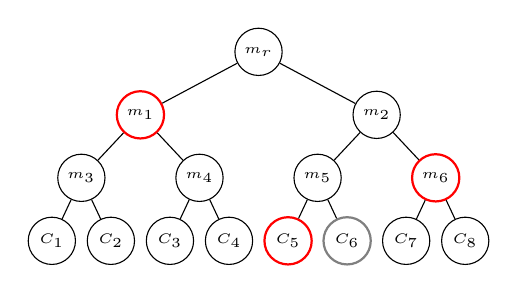
\begin{tikzpicture}[
    level 1/.style={sibling distance=30mm, level distance=8mm},
    level 2/.style={sibling distance=15mm, level distance=8mm},
    level 3/.style={sibling distance=7.5mm, level distance=8mm},
    every node/.style={draw, circle, minimum size=6mm, inner sep=0pt, font=\tiny}
]
    % Root node
    \node {$m_r$}
        % Level 1
        child {node[draw=red, line width=0.8pt] {$m_1$}
            % Level 2
            child {node {$m_3$}
                % Level 3
                child {node {$C_1$}}
                child {node {$C_2$}}
            }
            child {node {$m_4$}
                % Level 3
                child {node {$C_3$}}
                child {node {$C_4$}}
            }
        }
        child {node {$m_2$}
            % Level 2
            child {node {$m_5$}
                % Level 3
                child {node[draw=red, line width=0.8pt] {$C_5$}}
                child {node[draw=gray, line width=0.8pt] {$C_6$}}
            }
            child {node[draw=red, line width=0.8pt] {$m_6$}
                % Level 3
                child {node {$C_7$}}
                child {node {$C_8$}}
            }
        };
\end{tikzpicture}
\caption{Merkle tree with authentication path (in red) for commitment $C_6$ (in gray)}
\label{fig:merkle-tree}
\end{figure}

\subsection{Privacy-preserving blockchains}
\noindent Beneath the application layer there are blockchains utilizing zero-knowledge properties of SNARKs for infrastructural privacy preservation. For each transaction submitted, such systems must obscure the source, relevant currencies, amounts used, and payment recipients. Zerocash \cite{zcash} is a notable example of a network that does such a thing. Intended to be a privacy-preserving version of Bitcoin \cite{bitcoin}, Somewhat similar to (and preceding) Tornado Cash, Zerocash the unspent-transaction-output (UTXO) model, where transactions create so-called ``unspent funds'' that the party who ``owns'' them is entitled to spend. When they do spend those funds, another record of ``unspent funds'' for the recipient of the spending is created. These UTXO records are stored in a merkle tree, and spending funds requires proving knowledge of a leaf in the tree corresponding to the funds. Early versions of Zerocash used groth16 for this, but the NU5 upgrade of 2022 switched to the universal halo2 proof system \cite{halo2}, which enables a combination of a PlonK-style arithmetization and Bulletproofs-style commitment scheme \cite{bulletproofs} requiring no trusted setup at the expense of verifier performance.

\subsection{Verifiable Virtual Machines (VVM)}
\noindent Multiple ``Zero-knowledge virtual machines'' (zkVMs) \cite{scrollzkevm, polygonzkevm, sp1, risc0, openvm} have emerged as architecture-specific and general solutions for proving validity of layer-2 transaction batches on the layer 1 (L1) chains settling them. We use the more accurate phrase ``verifiable virtual machine'' (VVM) since succinctness is a higher priority than zero-knowledge in most L2 architectures. Sitting at the execution layer of the blockchain node implementation, the VVM is responsible for executing calls to smart contracts, generating corresponding execution traces/witnesses, and generating proofs of correct execution for each batch of transactions. PlonK-style variants have been a popular first approach due to the diverse computation structure and lookup-style arguments for verifying ``SNARK-unfriendly'' operations. Many VVM implementations use circuit domain-specific languages (DSLs) like halo2 to implement the circuits constraining the computation details. \\

% \noindent A crucial point of consideration here is that not all computations performed in VVMs are ``SNARK-friendly''; a prime example of this is hash functions like SHA256 which use non-linear or non-algebraic operations like bit mixing. This can cause the circuits constraining this computation to be overly complex and inefficient. To meet this end, lookup-based methods are of great interest here since they can avoid constraining ``SNARK-unfriendly'' operations directly without losing soundness. An example of this is lies in the proof for validity of transaction that called a contract function using \texttt{sha256()}. Instead of constraining the exact sha-256 computation, the prover and verifier would agree on a publicly known table of acceptable inputs and outputs for SHA-256, which the prover commits to as part of the proof. The verifier does not need to know the whole table - they just need to know a commitment to the one considered correct. This can then be compared with what the prover committed to.\\
